\section{Ejercicio 4}

El ejercicio consiste en implementar el scheduler $Round-Robin$, que soporte migraciones entre núcleos y tenga una única cola global
para los procesos. \\

Para esto se utiliza la estructura $queue<int>$, donde cada elemento de la misma representa un pid de algún proceso listo para ser ejecutado.
También se debe guardar la cantidad de cores y sus respectivos quantums, que son pasados como parámetro cuando se llama al constructor de la clase. 
Se almacenan entonces estos datos y el quantum que le queda a cada proceso en cada CPU, usando dos estructuras de tipo $vector<int>$.\\

Los métodos a implementar son:
 
$load(pid)$: encola $pid$ en $colaReady$ que es la cola de procesos en estado ready.
$unblock(pid)$: hace la misma acción, encolar nuevamente el pid de la tarea que se desbloqueó. Es decir, la tarea queda al final de la $colaReady$
En el método $tick(cpu, motivo)$ se toman 3 casos: el proceso consumió todo el ciclo usando el CPU, realizó una llamada bloqueante o terminó
 de ejecutarse. \\

\begin{itemize}
\item TICK: Si la tarea era IDLE_TASK y no hay procesos en $colaReady$ sigue ejecutando lo mismo.
			Si la tarea era IDLE_TASK pero hay tareas disponibles en $colaReady$ se toma el tope de la cola (se quita de la cola), se actualiza el quantum disponibles
			 y se devuelve ese pid.
			Si era cualquier otra tarea se resta un tick al quantum actual. Se chequea si se agotó su quantum, sino sigue ejecutando. Si lo consumió todo, se encola 
			el pid en colaReady, se actualiza el quantum diponible, y se toma el tope de la cola como pid siguiente.
\item BLOCK: Si no hay mas tareas en colaReady, se devuelve IDLE_TASK.
				Si hay, se actualiza el quantum diponible se devuelve el tope de colaReady quitando el elemento de la misma.
\item EXIT: Ídem BLOCK.
\end{itemize}

Se creó un lote de tareas con el fin de probar el correcto funcionamiento del scheduler.

\begin{itemize}
\item *2 TaskCPU 20
\item TaskConsola 10 1 5
\item TaskBatch 15 5
\end{itemize}


\begin{figure}[h]
  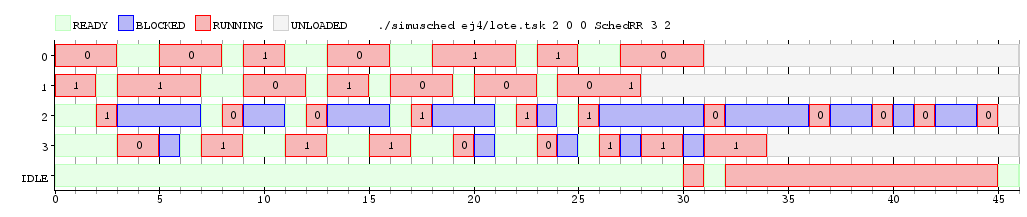
\includegraphics[width=\textwidth]{../ej4/test.png}
  %~ \caption{}
\end{figure}


En el gráfico se puede ver, como las tareas van migrando de núcleo, y que cada núcleo tiene un quantum asociado. En particular el core 0 tiene quantum 3 y el 
core 1 tiene como quantum 2. Cada vez que cada tarea agota su tiempo es desalojada y encolada en $colaReady$.
Cuando las tareas 2 y 3 realizan llamadas bloqueantes, son desalojadas y quitadas de la $colaReady$, una vez que se desbloquean se encolan nuevamente en $colaReady$
En el instante 5 se ve que como las tareas 2 y 3 estan bloqueadas la tarea 1 obtiene el cpu dos veces seguidas, ya que no queda ninguna otra tarea para ejecutar.
